\setcounter{page}{1}
\chapter{Theory}
The microscopic rolling motion of a bead in the magnetic flow cytometer is a mixture from continuum and classical mechanics. Introducing a biofunctionalization to the microchannel adds further complexity to a conglomerate of inertia, viscous and body forces. In order to identify the dominant actors and predict experiments qualitatively, an overview over all forces will be given in the theoretical background. The schematic directions of the respective contributors are shown in \cref{fig:theo:figOne}. For a subsequent equilibrium hypothesis, hydrodynamic phenomena such as the Saffman-, Magnus- or F\aa{}r\ae{}us-Lindquist effects are explained. Moreover, buoyancy and fluid drag as well as the resulting fluid-induced wall- and shear-lift forces are defined. Most importantly, however, are the electro-magnetic and biomolecular bond forces which are considered to be predominant in this system.(\cref{sec:theo:force})\\
Further, to corroborate some developed protocols of this thesis, a bio-chemical background will be motivated and introduced for covalent surface modifications in \cref{sec:theo:chem}. Special focus lies on wet-chemical surface oxidation, silanization and carbodiimide coupling chemistry. Thereover, the main measurement principle of the utilized magnetic flow cytometer has already been characterized exhaustively by \citet{lit:thes:helou}, \citet{lit:thes:reisbeck} and others.\cite{lit:thes:esthi,lit:thes:brenner} Nevertheless, key components and the measurement readout will be discussed in \cref{sec:theo:magnet}.
\begin{figure}[!htb]
	\centering
	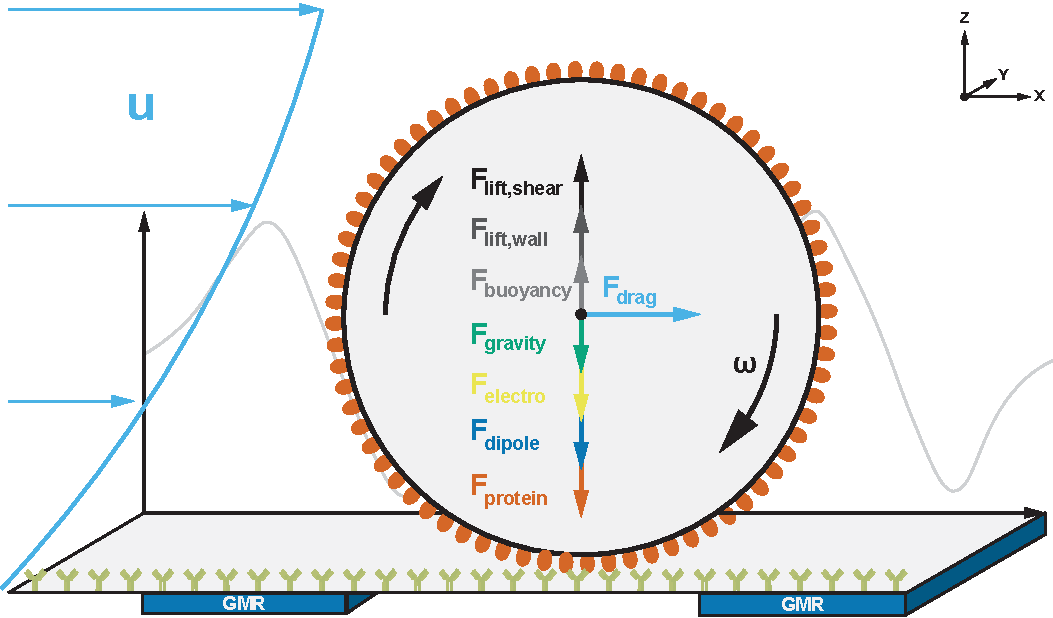
\includegraphics[width=.75\linewidth]{Ressources/Fluidic/FigureOne}
	\capption{Schematic Force Balance on a Rolling Particle with Bio-Functionalization}{The rolling motion of a microbead over the biofunctionalized surface of a microchannel is a mixture from continuum and classical mechanics. In order to identify the dominant actors and predict experiments qualitatively, an overview over all forces will be given in the theoretical background. The during the course of this thesis consistently used coordinate system was defined by $e_x$ in rolling direction. $e_z$ indicates the height, whereas $e_y$ specifies a width or depth.}
	\label{fig:theo:figOne}
\end{figure}

\section{Microfluidics}

\subsection{Incompressibility of Fluid Flows}

\label{sec:theo:incomp}

The main experiments of this work were carried out in microfluidic environments, which exhibit favorable properties compared to common macrofluidic systems. The governing rules of fluid mechanics change with respect to scale. In a microfluidic system interfacial as well as electrokinetic phenomena are predominant, and reduce the importance of pressure and gravity.\cite{lit:fluidic:kirby} However, electrodynamics, chemistry and fluid dynamics are inextricably intertwined. In effect, fluid flow can create electric fields (and vice versa), with a degree of coupling driven by the surface chemistry. Many of the resulting phenomena can be deduced from the conservation of mass described by the continuity equation (\cref{eq:continuityM}), the conservation of momentum described by the Cauchy-Momentum equation (\cref{eq:cauchymomentum}), and the resulting Navier-Stokes equation (\cref{eq:navierstokes}).\footnote{The mathematical prerequisites and notation for all following derivations are explained in \cref{sec:app:mathnot}}

\begin{align}
	\frac{\partial}{\partial t} \iiint \rho \ \mathrm{dV} &= - \iint \rho \mathbf{u} \cdot \vv{n} \ \mathrm{dA} \label{eq:continuityM}\\
	\nabla \cdot \mathbf{u} &= 0 \label{eq:conservMass}\\	
	\frac{\partial}{\partial t} \iiint \rho\mathbf{u} \ \mathrm{dV} &= - \iint \rho \mathbf{u}\mathbf{u} \cdot \vv{n} \ \mathrm{dA} + \iint \boldsymbol{\tau} \cdot \vv{n} \ \mathrm{dA}  + \iiint  \sum_\text{i}\mathbf{F}_\text{i} \ \mathrm{dV} \label{eq:continuityP} \\	
		\rho \frac{\partial \mathbf{u}}{\partial t} + \rho\mathbf{u} \cdot \nabla \mathbf{u} &= \nabla \cdot \boldsymbol{\tau} + \sum_\text{i}\mathbf{F}_\text{i} \label{eq:cauchymomentum} \\			
\end{align}
The foremost assumption in fluid dynamics is termed ``incompressibility''. Here, density gradients are negligibly small to assume a uniformity thereof. This leads to a significant simplification of the conservation equations, because any transfer from kinetic to internal energy can be ignored.\footnote{For sake of completeness, it should be mentioned that viscous forces can also transfer energy irreversibly to internal energy. However, they are inversely proportional to the system's size, and hence omitted.}
This continuity equation states that the mass of a control volume - in this case the volume integral over the \gls{rho} - can only change by the mass flux over its \gls{surfnormal} transported by the \gls{u}. For constant \gls{rho} the mass does not change over time. This finding and the application of Gauss's theorem (\cref{eq:Gauss}) yield the conservation of mass in an incompressible fluid. (\cref{eq:conservMass})


\subsection{Flow and Shear in Microchannels with Viscous Fluids}
\label{sec:theo:flow_and_Shear}

The above equation and Gauss's theorem can now be applied to the conservation of momentum relation. (\cref{eq:continuityP}) Integration then yields the Cauchy momentum equation which states that any change in momentum inside a control volume ($\rho \frac{\partial \mathbf{u}}{\partial t}$) is caused by convective transport from or to the volume ($\rho\mathbf{u} \cdot \nabla \mathbf{u}$), surface stresses ($ \nabla \cdot \boldsymbol{\tau}$), and the volumetric net \gls{bodyforce} such as gravity or electrostatics.

Hereby, the \gls{tau} can be further decomposed into the \gls{tau_p} and \gls{tau_v} as shown in \cref{eq:surfaceStressTensor}. Characteristically, the pressure related contributions act normal and independently from \gls{u} whereas viscous forces act normal and tangential, and are dependent on \gls{u}. The \gls{tau_p} can therefore be expressed by a scalar pressure acting in every spatial dimension, which is mathematically represented by the identity. 
\begin{align}
	\boldsymbol{\tau} &= \boldsymbol{\tau}_\text{viscous} +  \boldsymbol{\tau}_\text{pressure} = 2\eta \boldsymbol{\epsilon} - p \mathbf{I}_\text{\scaleto{3 \times 3}{4pt}} \label{eq:surfaceStressTensor}\\
	\nabla \cdot \boldsymbol{\tau}_\text{viscous} &= \nabla \cdot 2\eta \boldsymbol{\epsilon} = \nabla \cdot \eta \nabla \mathbf{u} \underset{\text{uniform}}{\overset{\text{only \ if \ }\eta}{=}} \eta \nabla^2 \mathbf{u} 	\label{eq:divergence_Stresstensor} \\
	\aunderbrace{\vphantom{\sum_{i}} \rho \frac{\partial \mathbf{u}}{\partial t}}_{\text{Transient}}\ +\ \aunderbrace{\vphantom{\sum_{i}}\rho\mathbf{u} \cdot \nabla \mathbf{u}}_{\text{Convection}}\ &=\ \aunderbrace{\vphantom{\sum_{i}}-\nabla p}_{\text{Pressure}}\ +\ \aunderbrace{\vphantom{\sum_{i}}\eta \nabla^2 \mathbf{u}}_{\text{Viscous}}\ + \aunderbrace{\sum_{i}\mathbf{F}_\text{i}}_{\text{Body \ Forces}} \label{eq:navierstokes}
\end{align}

The viscous stresses however can not be described by a continuum equation, but only by a constitutive relation of atomistic processes. The fundamental model of Newton's mechanics assumes that the \gls{eta} is neither dependent on any velocity nor on the strain rate. Therefore, fluids which satisfy this condition are called \textit{Newtonian} fluids. Omitting special \textit{Non-Newtonian} cases such as shear-thinning, -thickening or complex colloidal fluids such as undilute blood, \gls{eta} is the scalar proportionality that relates the strain rate to surface stress.\cite{lit:fluidic:kirby} This is captured in the equation $\boldsymbol{\tau}_{viscous} = 2\eta \mathbf{\epsilon} $. Thereby, the \gls{epsilon} is part of the decomposition of an unidirectional flow field. It resembles on the one hand any stretching or squeezing of fluid by \textit{extensional strain} and on the other hand \textit{shear strain} which is responsible for skewing.\cite{lit:fluidic:kirby}

The divergence of \gls{tau_v}, as used in the incompressible Cauchy momentum equation (\cref{eq:cauchymomentum}), can be further simplified with \cref{eq:divergence_Stresstensor} by taking advantage of the anti-transpose symmetry of the flow field.\cite{lit:fluidic:kirby} If \gls{eta} is also uniform and isotropic across the channel, the scalar viscosity can be extracted from the divergence.  Applying all assumptions to the Cauchy momentum equation (\cref{eq:cauchymomentum}) yields as final result the \gls{nse}. (\cref{eq:navierstokes}) 

However, the \gls{nse} has no analytic solution yet and can in consequence only be solved for defined boundary problems. The two most common boundary conditions herefore are the ``no-penetration condition'' ($\mathbf{u} \cdot \vv{n} = 0$) and the ``no-slip condition'' ($\mathbf{u}_t = \mathbf{u} - (\mathbf{u}\cdot \vv{n}) \vv{n} = 0$), which state that the normal and tangential components of fluid velocity are per definition zero at motionless, impermeable walls.\newline
Alongside these conditions, many problems arise due to turbulent flow and therefor transient effects. Mathematically, this can be avoided by simply neglecting the time-dependent term in the \gls{nse}. For viscosity dominated flow it can be argumented that fluid moves in isoplanar \textit{lamina}\footnote{latin: lamina = plate, sheet, foil}. In experimental observations, these laminar flows then proved to be steady to perturbations.

\begin{equation}
	\mathit{Re}\ =\ \frac{\mathrm{\mathsf{fluid\ density\ \times \ velocity\ \times\ size}}}{\mathrm{\mathsf{viscosity}}} \label{eq:reynolds}
\end{equation}

In a first order approximation, the dimensionless \gls{re}, which compares the inertia to viscous forces, allows a qualitative prognosis about the flow regime. (\cref{eq:reynolds}) A reynolds number below a threshold of 2300 indicates laminar flow in Hagen-Poiseuille flows. This holds true for the utilized microfluidic with the dimensions \SI{15800}{\micro\meter} $\times$ \SI{700}{\micro\meter} $\times$ \SI{150}{\micro\meter} (\gls{chanL} $\times$ \gls{chanW} $\times$ \gls{chanH}) and aequous buffer solutions. Typically, where smallest length \gls{chanH} or the hydraulic diameter is considered as \textit{characteristic size}, whereas the characteristic velocity is usually employed by either the maximum of \gls{u} or \gls{umean}. With the smallest length and the mean flow, \gls{re} equals \num{2.1399} for a \gls{q} of \SI{80}{\micro\liter\per\minute} (\gls{chanH} = \SI{150}{\micro\meter}), whereas for a \gls{q} of \SI{8}{\micro\liter\per\minute} (\gls{chanH} = \SI{50}{\micro\meter}) the \acrlong{re} already drops to \num{0.214}.  Hence, several fluidic phenomena such as deterministic pathlines as well as simplifications of the \gls{nse} can be exploited in the present system. 

In the model case of a flow through a rectangular channel, no analytical solution of the \gls{nse} exists. A Fourier Series expansion - if the width is larger than height of a channel - can solve the problem with sufficient precision as shown in \citet{lit:fluidic:bruus}. Equation \cref{eq:flowVelocityRect} determines the magnitude of the flow field parallel to the pressure gradient in relation to the horizontal coordinate $y$ and vertical coordinate $z$ with respect to \gls{chanW} and \gls{chanH}. An integration over the flow field in the channel cross section yields the \gls{q}. (\cref{eq:flowRateRect})\footnote{The equation \cref{eq:flowVelocityRect} shows that height deviations can have prominent influence on a channel velocity simulation as it is proportional to $h^2$. Further, the flow rate depends even on $h^3$.} 

  \begin{align}
\mathbf{u}   _x(y,z) &= \frac{4 h^2 \Delta p}{\pi^3 \eta l} \sum_{n,\text{odd}}^{\infty} \frac{1}{n^3} \left( 1- \frac{\cosh (n \pi \frac{y}{h})}{\cosh (n \pi \frac{w}{2h})} \right) \sin (n \pi \frac{z}{h}) \label{eq:flowVelocityRect} \\
  Q    &= \int_{-\frac{1}{2}w}^{\frac{1}{2}w} \int_{0}^{h} u   _x(y,z) \ \mathrm{dzdy} \approx \frac{h^3 w \Delta p}{12 \eta l} \left( 1 - \frac{h}{w}) \right) \label{eq:flowRateRect} \text{, \ for \ } h < w
\end{align}


\subsection{Force Equilibrium of Microbeads}
\label{sec:theo:force}
Although microfluidic systems mostly operate in a low inertia regime as specified by low \gls{re}, the force equilibrium $\sum_{i} \mathbf{F} \overset{!}{=} 0$ and subsequently the velocity of any particle in the fluid stream is influenced as it moves closer to the boundaries. Several models have already been implemented with a part of the mentioned forces. \citet{lit:fluid:comparison} compared the importance of translation, rotation and shear forces. \citet{lit:fluidics:RollingCharacteristics} evaluated cell rolling characteristics, and \citet{lit:fluidic:ModelMIT} proposed a model for bead-based immunoassays in microfluidics. Therefore, an overview over all (inter-)acting forces shall be given here.

\begin{equation}
	\mathit{Re}_\text{particle} = \frac{r^2}{\frac{2wh}{w+h}} \ \mathit{Re} 
\end{equation}

Additionally to the channel Reynolds number \gls{re}, describing the ratio between inertial force and viscous force of fluid in a flow, \citet{lit:fluidic:f_wall} proposed a \gls{re_p} considering the size ratio of particle to channel. At \gls{re_p} $\ll 1$, particles are subjected to the dominant viscous drag to follow fluid streamlines. In the contradictory case, inertia becomes prominent. On increasing \gls{re_p} to the order of 1, inertial lift forces become dominant and lateral migration of particles across streamlines becomes visible.  For a micrometer sized bead and a channel as referred to in \cref{sec:theo:flow_and_Shear}, the pre-factor is in the range of \numrange{1e-5}{1e-7} hence viscous drag overweighs inertial lift of a particle.

\subsubsection{Stoke's Drag}
\vspace{\baselineskip}
\begin{figure}[!h]
	\subfloat{
		\subfigimg[height=50pt]{a}{./Ressources/Fluidic/drag}	
		\phantomsubcaption
		\label{fig:fluidic:drag}
	}
	\hfill
	\addtocounter{subfigure}{-1}
	\subfloat{
		\subfigimg[height=50pt]{b}{./Ressources/Fluidic/lift1}
		\phantomsubcaption
		\label{fig:fluidic:lift1}
	}%
	\hfill
	\addtocounter{subfigure}{-1}
	\subfloat{
		\subfigimg[height=50pt]{c}{./Ressources/Fluidic/lift2}
		\phantomsubcaption
		\label{fig:fluidic:shear}
}
	\capption{Particle Drag and Lift Behavior}{(\textbf{a}) Bulk Drag: Force acts on a particle caused by the displacement of fluid stream lines. (\textbf{b}) Wall-lift Drag Force: In a special case of drag, where streamlines cannot be displaced further, a pressure gradient forms in front of the sphere. This forces a motion directed perpendicularly from the wall. (\textbf{c}) Shear-induced force: The curvature of the flow profile exhibits a translation and rotation due to inhomogeneously distributed shear on the surface.\cite{lit:fluidic:imageLift}}
	\label{fig:fluidic:lift}
\end{figure}
\begin{align}
	\mathbf{F}_\text{drag,wall} &= -6 \pi \eta r \ \overline{\mathbf{u}} \ C \label{eq:f:drag}\\	
	C_\text{drag} &= \frac{24}{Re} \left( 1 + 0.15Re^{0.687} \right) \label{eq:f:drag:corr:bulk} \\
	C_\text{drag,exact} &=  \frac{4}{3} \sinh \alpha \sum_{n=0}^{\infty} \left(\frac{n(n+1)}{(2n-1)(2n+3)} \ \cdot \ A \right) \label{eq:f:corr:wall_exact}\\
	\alpha &= \cosh^{-1}\frac{z}{r}, \\ A &= \frac{2 \sinh((2n+1)\alpha) + (2n+1)\sinh2\alpha}{(2\sinh((n+0.5)\alpha))^2 -((2n+1)\sinh\alpha)^2 }-1\\
	C_\text{drag,wall} &= \frac{1}{1 - \frac{9}{16}\frac{r}{r+z} +\frac{1}{8}\left(\frac{r}{r+z}\right)^3 - \frac{45}{256}\left(\frac{r}{r+z}\right)^4 - \frac{1}{16}\left(\frac{r}{r+z}\right)^5} \label{eq:f:drag:corr:wall_approx} \\ \mathbf{F}_{\text{drag,wall,}\perp } &= \frac{6 \pi \eta r \overline{\mathbf{u}}}{1 - \frac{9}{8} \frac{r}{r+z} + \frac{1}{2} \left( \frac{r}{r+z} \right) ^{3} }  \label{eq:f:drag:per:wall} \\
%	v_z &= \frac{3}{64} \mathit{Re}_\text{s} \mathbf{u}_\text{s} \ = \ \frac{3}{64} \frac{\rho_\text{fluid} z \mathbf{u}_\text{s}}{\eta} \mathbf{u}_\text{s} \ , \ (\frac{\rho_\text{fluid} z \mathbf{u}_\text{s}}{\eta}) \ll 1 \label{eq:repulsion_v}\\
	\omega &= \frac{3 \mathbf{u}}{32 r}\left(\frac{r}{r+z}\right)^{4}\left(1-\frac{3}{8} \frac{r}{r+z}\right) \mathrm{, \ for \ } (\frac{r}{r+z})^2 \ll 1	\label{eq:f:drag:angularFreq}
\end{align}
The foremost force to actuate particles inside a microfluidic channel is \gls{f:drag}.(\cref{eq:f:drag}) It originates from additional flow resistance caused by a particle in the channel cross section. The fluid therefor displaces its elements in orthogonal to the movement direction.\cite{lit:fluidic:motion_sphere_to_plane_surface}  In the interfacial perspective, viscous fluid is moving past the sphere surface with an axial velocity difference. On the boundaries, a slip condition has to be applied. This is illustrated by a particle with the surrounding streamlines for the bulk case in \cref{fig:fluidic:drag}, and for adjacent walls in \cref{fig:fluidic:lift1,fig:fluidic:shear}. In the bulk, due to the no-slip boundary as first order approximation, a drag can be not only expressed by the viscous fluid force \gls{u} $\times$ \gls{eta} on a circular surface boundary ($2r\pi$) but has to be scaled in low \gls{re} regimes by \cref{eq:f:drag:corr:bulk} to account for skin friction and form drag.

In the proximity of a channel wall, however, where on one side no fluid can be displaced further, another correction factor was deduced by \citet{lit:fluid:Hydrodynamics}, based on works of Faxs\'{e}n and Oseen, that increases the drag in parallel direction non-linearly.(\cref{eq:f:corr:wall_exact}) A phenomenological approximation of the correction factor yields equation \cref{eq:f:drag:corr:wall_approx}, when viscosity dominates the difference. with an error of $\mathcal{O}\left((\frac{r}{r+z})^7\right)$.\cite{lit:fluid:velocities, lit:fluidic:motion_sphere_surface_2009} 

Additionally, the viscous drag force causes an induced secondary flow which leads to a perpendicular lift force (\cref{eq:f:drag:per:wall}).\cite{lit:fluid:Hydrodynamics,lit:fluidic:kim} This leads to a great influence in purely inertia-dominated or multi-phase flows.\cite{lit:fluid:deformabilityDiCarlo}  Adopted to an example, a spherical air-bubble inside a water flow feels only \SI{67.4}{\percent} of the drag by surrounding fluid.

\begin{figure}[!htb]
	\subfloat{
		\subfigimg[height=120pt]{a}{./Ressources/Fluidic/RotationSpheredistant}
		\phantomsubcaption
		\label{fig:fluidic:particleRotationfar}
	}%
	\hfill	
	\addtocounter{subfigure}{-1}
	\subfloat{
		\subfigimg[height=120pt]{b}{./Ressources/Fluidic/RotationSpherenear}
		\phantomsubcaption
		\label{fig:fluidic:particleRotationnear}
 	}
	\capption{Particle Rotation Behavior}{(\textbf{a}) Direction of rotation of
		a sphere settling in eccentric position	between parallel walls. (\textbf{b}) Direction of rotation of a sphere settling in the presence of a single plane wall far from the other side.\cite{lit:fluidic:f_wall}}
	\label{fig:fluidic:particleRotation}
\end{figure}
The considerations of \acrlong{f:drag} above were limited for linear translation cases. Nevertheless, fluid drag also imposes a non-negligibly torque on particles if a particle moves nearer than 10 diameters to the wall. \citet{lit:fluid:Hydrodynamics} mention an experimentally determined formula in \cref{eq:f:drag:angularFreq} to calculate a drag-related \gls{omega_freq}. Counter-intuitively, the direction of rotation in the bulk fluid (\cref{fig:fluidic:particleRotationfar}) is opposite than from the rotation direction near or touching the wall (\cref{fig:fluidic:particleRotationnear}). This can be explained by a complex superposition of tangential components from later mentioned forces and will not be explained to any more extent here.\cite{lit:fluid:Hydrodynamics,lit:fluid:comparison}

\subsubsection{Gravity and Buoyancy}
On every mass in our environment acts \gls{f:grav} to pull it along its gradient. In a medium, notwithstanding, it is balanced by the displacement of the same in the counter-direction called \gls{f:buoyancy}. As a microparticle made from a co-polymer - especially when it carries magnetic momentum - has a significantly higher density than water, \gls{f:grav} (\cref{eq:f:grav}) outperforms \gls{f:buoyancy} (\cref{eq:f:buoyancy}), which in term causes a particle to sink to the channel floor.
\begin{align}
	\mathbf{F}_\text{buoyancy} &= -\frac{4}{3}\pi r^3 \ \rho_\text{fluid} \ g \label{eq:f:buoyancy}\\
	\mathbf{F}_\text{gravity} &= +\frac{4}{3}\pi r^3 \ \rho_\text{particle} \ g \label{eq:f:grav}
\end{align}


\subsubsection{Magnetic Force}
The - during the course of this thesis - strongest acting force is exhibited by the \gls{B}, which acts on paramagnetic particles with a \gls{m}.\cref{lit:bio:attomolarDetection} When an external magnetic field is non-uniform, there will be a \gls{f:mag}, proportional to the magnetic field gradient, acting on the \gls{m}.(\cref{eq:f:mag}) For particles that carry magnetite or similar ferrimagnetic material in their polymer shell, the magnetic momentum can be inferred by the integration of \gls{M}: $\mathbf{m} = \int\int\int \mathbf{M} \text{dV}$. However, the more unified approach is a comparison of \glspl{chi} as described in \cref{eq:f:mag} which involves also diamagnetism and negative magnetophoresis. Consequently, if the particle susceptibility is greater than the fluid's, a microbead will move towards the field maximum. Calculated for an \SI{8}{\micro\meter} bead with \SI{1.12e-12}{\ampere\meter\squared} saturation magnetization, \gls{f:mag} results in \textasciitilde{}\SI{45}{\pico\newton} for a typical field gradient of \SI{5}{\tesla\per\meter}.
\begin{align}	
	\mathbf{F}_\text{mag} &=\frac{V_{p}\left(\chi_{p}-\chi_{f}\right)}{\mu_{0}}(\mathbf{B} \cdot \nabla) \mathbf{B} \label{eq:f:mag}	\\
	\mathbf{F}_\text{dipole} &=\left(\mathbf{m}\cdot \nabla \right) \mathbf{B} = -\nabla \mathbf{E}_\text{dipole}\\
	\mathbf{E}_\text{dipole}&=\sum_{i-1}^{n} \frac{\mu_{0}}{4 \pi r_{i}^{3}}\left(\mathbf{m}_{\mathbf{i}} \cdot \mathbf{m}_{\mathbf{ref}}-\frac{3}{|\mathbf{r}_{i}|^{2}}\left(\mathbf{r}_{\mathbf{i}} \cdot \mathbf{m}_{\mathbf{i}}\right)\left(\mathbf{r}_{\mathbf{i}} \cdot \mathbf{m}_{\mathbf{ref}}\right)\right)  \label{eq:f:dipole}
\end{align}
From a microscopic perspective, magnetic beads interact with each other according to the dipolar interaction. In that case, a reference bead with magnetic momentum $\mathbf{m}_{\mathbf{ref}}$ at distance $\mathbf{r}_{\mathbf{ref}}$ feels the force of all surrounding particles.(\cref{eq:f:dipole}) Bringing every dipole in a control volume in superposition leads to the overall magnetic dipole field and can operate as another pathway towards the \gls{f:mag} calculation.


\subsubsection{Electrostatic Interaction}
The microchannel - as well as a particle in it - carries an electrical double layer on the surface due to present surface charges. The net charge acquired by the particles can be computed by integrating the particles’ surface charge densities over their surfaces as described by Gauss’s Law. However, as \gls{f:el} on charge $q_1$ is square dependent of the distance from the secondary charge $q_2$ at the respective locations $\mathbf{r}_{1},\ \mathbf{r}_{2}$.(\Cref{eq:f:el}) This, and the fact that the surface net charge in a buffer solution is insignificant, lead to the assumption that \gls{f:el} plays a minor role in this force equilibrium. 

\begin{equation}
	\mathbf{F}_\text{el}=\frac{q_{1} q_{2}}{4 \pi \varepsilon_{0}} \frac{\mathbf{r}_{1}-\mathbf{r}_{2}}{\left|\mathbf{r}_{1}-\mathbf{r}_{2}\right|^{3}} \label{eq:f:el}
\end{equation}

\subsubsection{Magnus Lift Force}
\vspace{\baselineskip}
\begin{figure}[h!]
	\centering
	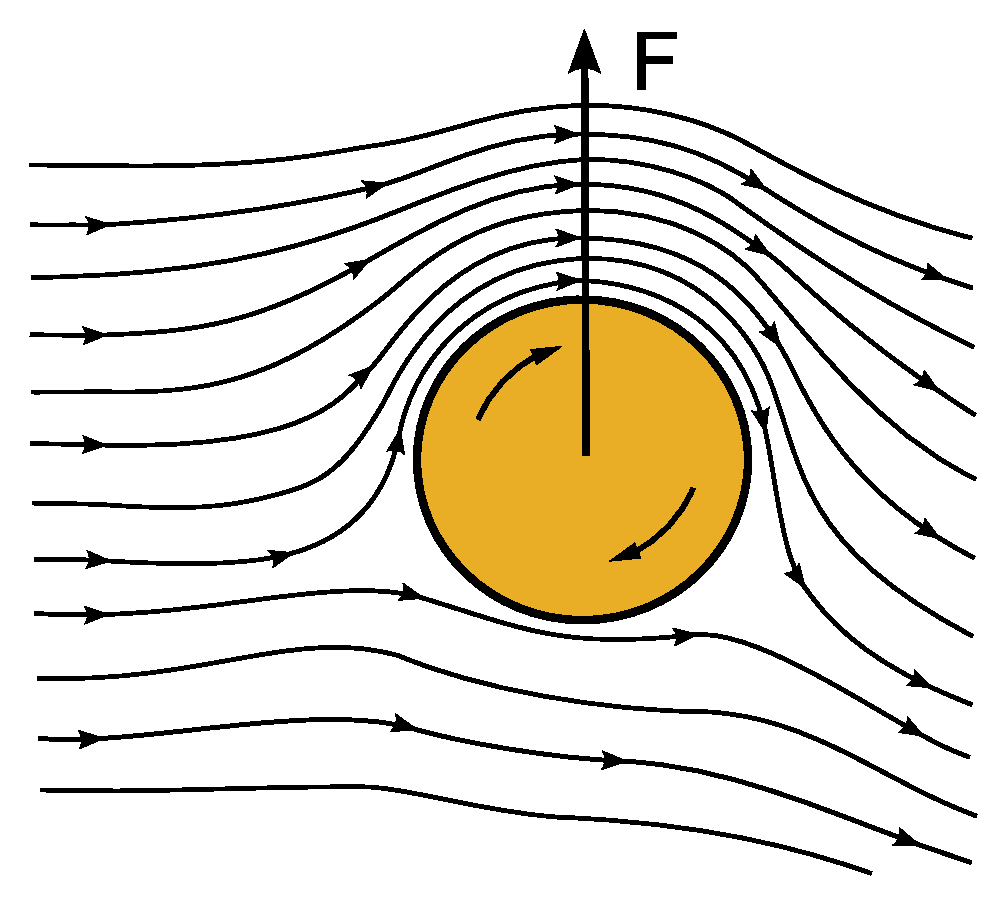
\includegraphics[width=0.6\linewidth]{./Ressources/Fluidic/Magnus-effect.pdf}
	\capption{Magnus Effect on a Particle in Laminar Flow}{The intrinsic rotation of a particle inside a laminar flow field causes a pressure gradient to the side whose tangential rotation vector is parallel to the stream lines.}
	\label{fig:fluidic:magnus}
\end{figure}
The \gls{f:magnus} is a rotation-induced variable as a result of the pressure difference induced by streamline asymmetry.\cite{lit:fluidic:inertialFluidicsForces} For a spinning particle in a fluid as shown in \cref{fig:fluidic:magnus}, the streamline density and therefor the pressure on the one side of the particle is lower relative to the other side. The main driver of this effect is again the no-slip boundary, where fluid on the front side of the particle is dragged down whereas the fluid on the bottom side is slowed down. As a result, this leads to a lift force perpendicular to the flow direction.
\begin{equation}	
	\mathbf{F}_\text{magnus} =  \frac{1}{8}\pi r^3 \rho_\text{fluid} \ ( \mathbf{u} \times \mathbf{\Omega}) \label{eq:f:magnus}
\end{equation}
\subsubsection{Saffman Lift Force}
When the rotation speed of a particle in shear rate direction is much greater, $\mathbf{\Omega}>12\nabla\mathbf{u}$, for a freely rotating particle \gls{f:saffman} will begin to act. Depending on the interaction of slip velocity and shear, it will counteract any movement to the planar surface. Hence, at high gradients the center of rotation causes a shift to the maximum shear. \newline 
Scaling with \gls{omega_freq}, it will generally be at least one order of magnitude larger than Magnus force. Especially for electically or magnetically actuated particles, \gls{f:shear} is more relevant in the case of non-neutrally buoyant spheres.\cite{lit:fluidic:inertialFluidicsForces} 
\begin{equation}	
	\mathbf{F}_{saffman} = \frac{81.2}{4} (\mathbf{u} - u_p) r^2 \sqrt{\frac{\rho_{fluid}}{\eta} \nabla \mathbf{u}} \label{eq:f:saffman}
\end{equation}

\subsubsection{Shear-induced Lift Force}
This force is caused through a curvature in the flow profile and hence an inhomogeneously distributed shear over the sphere cross-section. Following the flow profile, \gls{f:shear} causes particles to migrate toward walls until the wall lift force repels and balances it. In contrast, if the curvature of \gls{u} is zero, it collapses to a simple shear flow. Then, the pressure will increase off-axis and start pushing particles to the centerline. As shown in \cref{fig:fluidic:shear} the magnitude of \gls{u} is much higher on the wall-distant side, due to the parabolic nature of the flow profile. Similar to \gls{f:saffman},  the  dissymmetry  of  relative  velocity  causes  a  lower  pressure  on the wall side, generating a shear gradient lift force which is opposite to the Saffman force.\cite{lit:fluidic:inertialFluidicsForces} 
\begin{equation}	
	\mathbf{F}_\text{shear} = K \rho_\text{fluid} (\nabla \mathbf{u})^2 r^4\ \text{, \ with\ } K \ \text{ from }\  \cref{eq:f:drag:corr:wall_approx} \label{eq:f:shear}
\end{equation}

\subsubsection{Deformability-Induced Lift Force}
Although rigidity can be assumed in the first order to study the hydrodynamic behavior of particles in a microchannel, cells and vesicles are deformable in real experiments. The deformability  will  induce an additional  lift  force on the particles, which is perpendicular to the main streamline, and is subjected nonlinearities  caused  by  the matching   of   velocities   and   stresses   at   the   deformable   particle interface. 

\begin{align}
	\mathbf{F}_\text{deformation}&=\mu \mathbf{u} r \left(\frac{r}{h}\right)^{2} \frac{r+z}{h} f\left(\lambda\right) \label{eq:f:deform}\\
	f(\lambda) &=\frac{16 \pi}{\left(\lambda+1\right)^{3}}\left[\frac{11 \lambda+10}{140}\left(3 \lambda^{3}-\lambda+8\right)+\frac{3}{14} \frac{19 \lambda+16}{3 \lambda+2}\left(2 \lambda^{2}-\lambda-1\right)\right] 
\end{align}

For example, deformability-induced  lift  force  has  been  used  already to  separate  and  enrich  malaria-infected \gls{rbc}  from  normal  healthy  \gls{rbc} for  the  diagnosis  of  malaria.  The parasite releases proteins that trigger the cross-linking of the spectrin network of the membrane, thus increases the rigidity of the infected cells.\cite{lit:fluid:deformability}
\citet{lit:fluid:deformabilityDiCarlo} reported a parallelized  microfluidic  device  that  passively separates pathogenic bacteria from the diluted blood by the use a unique differential transit time due to channel height differences which in turn caused size-dependent inertial  lift forces to obtain cell separation.

\subsubsection{F\aa{}r\ae{}us and F\aa{}r\ae{}us-Lindquist Effect}
\label{sec:theo:faraeus}
Often confused, the F\aa{}r\ae{}us and F\aa{}r\ae{}us-Lindquist effect constitute two different hemodynamic properties relevant for microfluidics with blood samples. Whereas the  F\aa{}r\ae{}us effect states that \glspl{rbc} are depleted in the wall regions of capillaries (due to the lift forces mentioned before), the F\aa{}r\ae{}us-Lindqvist effect describes the behavior of blood to decrease its viscosity in narrow channels.\cite{lit:fluid:faraeus, lit:fluid:faraeuslinquvist} Thereby, the latter effect is not solely driven by the first, but also the Segr\'{e}-Silberberg effect, who discovered that for neutrally buoyant particles an equilibrium at exact $0.6r$ from a tubing center forms.\cite{lit:fluid:silberbereffect} To model this effect, \citet{lit:fluid:cell-free-model} developed a cell-free marginal layer model.


\subsection{Rolling Motion and Surface Interaction of Beads}
\label{sec:theo:rolling}
Despite the fluid effects on a particle, the contact surface has also a significant influence on the movement of a particle. A fragile force equilibrium is necessary in order to achieve a stable rolling motion.\cite{lit:fluidic:wallInducedForces} Especially in geology, transient particle transport has been discussed intensely. There, two main termini are conventional: \textit{Contact load}, which identifies particles that move in contact with the bed by sliding or rolling over it, and \textit{saltation load}, which designates the movement as a series of “hops” along the bed, each hop following a ballistic trajectory. To elaborate this further, if a particle remains immobile to the flow and the velocity gradient is large enough so that the lift force exceeds the particle’s adhesive forces, it will jump in a steep trajectory from the channel bottom. Once off, the pressure difference from top to bottom of the particle is lost. Subsequently, it is carried downstream as it falls back to the bed following a ballistic trajectory of saltation.

\subsubsection{Contact Area of a Sphere and Flat Surface}
Once the acting forces brought the bead in contact with a wall or the channel bottom, it starts to move forward in a rolling motion. In a simple model, rolling on a plane without slipping is constrained by a sphere's translation ($\mathbf{F}_\parallel,\ \mathbf{F}_\perp$), rotation ($\omega$), and shear. Nevertheless, due to the rigid nature of the sphere, any shear will be omitted in further models.\cite{lit:fluid:rolling:rigid_viscoelastic} The no-slip boundary condition has to be applied also here by the requirement that the points of the sphere momentarily in contact with the plane are at rest. \newline However, rolling contact problems are dynamic because the contacting bodies are continuously moving with respect to each other. The contact patch in a sliding problem continuously consists of the same particles. In contrast, particles enter and leave the contact area during rolling. Moreover, in a sliding problem the surface particles in the contact patch are all subjected the same tangential shift everywhere, whereas in a rolling problem the surface particles are stressed in different ways. During rolling, they are free of stress when entering the contact, then stick to a particle of the opposing surface, and are strained by the overall motion difference between the two bodies, until the local traction bound is exceeded and local slip sets in.\cite{lit:fluid:rolling:contact_phenomena} \newline
In a real world, pressing two bodies with rough surfaces against each other limits the contact between the two bodies to a value, which is much smaller than the nominal contact area. Additionally, on natural and engineering surfaces Lennard-Jones potential, wetting, and molecular interactions start to play a role on the spectated microscale.\cite{lit:fluid:rolling:contact_ground_plane}

\begin{figure}[tbph!]
	\centering
	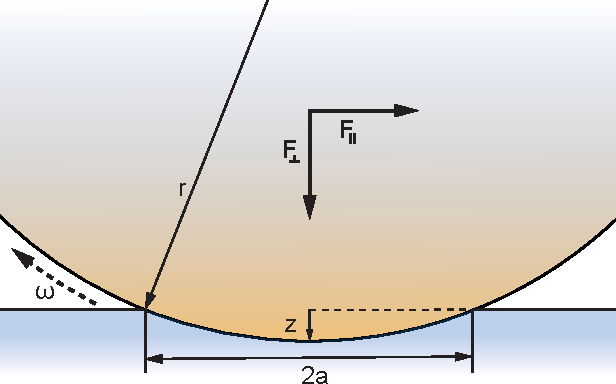
\includegraphics[width=0.7\linewidth]{Ressources/Fluidic/Rolling.pdf}
	\capption{Rolling Mechanics of a Sphere}{Penetration model of a sphere with radius $r$ adapted from \citet{lit:fluid:rolling:contact, lit:fluid:rolling:contact_ground_plane}. The top body moves into the elastic bottom body for an \acrfull{z} and a contact area $\pi a^2$.}
	\label{fig::fluidic:rolling_mechanics}
\end{figure}

In reality, with elastic effects taken into consideration, a different situation occurs. If an elastic sphere is pressed onto an elastic plane (ideally of the same material), both bodies deform and a Hertzian pressure distribution arises. The center of the sphere is moved down by an \gls{z} as shown in \cref{fig::fluidic:rolling_mechanics} that can also be desribed as ``maximum penetration distance''. It can now be calculated that the normal contact area between the bodies follows $A_{contact} = \pi a^{2}=\pi\left(2 r z-z^{2}\right)=2 \pi r z\left(1-\frac{z}{2 r}\right)$. Assuming that $z \ll 2r$ and considering that $A_{contact}$ must be zero for all $z < 0$, the following equation for the contact area arises. (\cref{eq:a_contact}) The spherical contact surface can be calculated analogous \Cref{eq:s_contact}.\cite{lit:fluid:rolling:contact_ground_plane}

\begin{align}
	A_{contact} &= 2\pi r z \mathrm{, \ for \ } z \geq 0 \label{eq:a_contact}\\
	S_{contact} &= \pi r (2z + a^2) = \pi z (4r - z)  \mathrm{, \ for \ } z \geq 0 \label{eq:s_contact}
\end{align}

For a \SI{8}{\micro\meter} microbead and a penetration depth \gls{z} of \SI{100}{\nano\meter} this yields for example an interaction with \SI{6.84}{\percent} of the total sphere and a total area of \SI{13.753}{\micro\meter\square}. Several methods and experiments have already been developed in the literature to measure the resulting friction and penetration parameters. A general model of a sphere in contact with a wall was optimized by \citet{lit:fluid:sphere_planeWall}. Experimentally, \citet{lit:fluid:rolling:contact} developed a microtribometer in PDMS to evaluate adhesion properties and validate their model's predictions.

\subsubsection{Protein interaction during Rolling}
In the attempt to mimic rolling adhesion on vascular surfaces which is the first step in recruiting circulating leukocytes and other cells into the tissue, protein-protein-interactions as driver for microbead motions have been studied extensively in this thesis. Statistically, a cell flowing near the vessel wall is able to attach if its adhesion receptors contact ligands on the wall. Bond formation, anyhow, involves distinct steps: transport, which brings two molecules into close proximity, and reaction, during which the molecules dock. Faster cell velocity produces more collisions but also limits the interaction time between interaction molecules. Thus, the relative timescales for transport and docking affect the efficiency of tethering a flowing cell to the surface.\cite{lit:bio:CellAdhesion}

\begin{figure}[!h]
	\subfloat{
		\subfigimg[height=150pt]{a}{./Ressources/Fluidic/dembo-model}		
		\phantomsubcaption
		\label{fig:fluidic:model:dembo}
	}
\hfill
	\subfloat{
		\subfigimg[clip,trim=0 1 0 0,height=150pt]{b}{./Ressources/Fluidic/model-voldman}
		\phantomsubcaption
		\label{fig:fluidic:model:voldman}
	}
\capption{Membrane Adhesion and Detachment Models}{(\textbf{a}) Adhesion Model after \citet{lit:fluidic:BindingPhysics}: Every interaction is viewed as spring-damper-model in superposition. (\textbf{b}) Surface Coverage Assay Model: In a stochastic approach, analyte molecules and their interactions are modeled between a planar and a spherical surface.  Adapted from \citet{lit:fluidic:ModelMIT}
}
\label{fig:fluidic:model}
\end{figure}

\citet{lit:fluidic:rollingWall}


For these properties, \citet{lit:fluidic:BindingPhysics} developed a detailed physical description of membrane adhesion and detachment kinetics. \citet{lit:fluidic:ModelMIT} then proposed an integrated model for bead based rolling mechanisms under the influence of protein interaction. The key for interaction thereby is the specific \textit{affinity} respectively \textit{avidity} of the protein and its ligand. In general, high-affinity ligand binding results from greater attractive ligand-receptor-forces and results in a higher tenancy of the receptor. However, lifetime of a formed complex does not correlate. The net ligand affinities are unitized by the \gls{kd}, which relates the reverse reaction rate (``the dissociation of the bond'') to the the forward reaction rate (``the formation of the bond''). Therefor high-affinity results in low \gls{kd}.\newline
On a bead and microchannel surface, however, not only one but multiple protein-ligand complexes are formed and dissociated simultaneously. This is described by \textit{avidity}. Though single binding events elevate the likelihood of other interactions, avidity is not relating the sum of its ingredient affinities but can rather be seen as the combined effect of all affinities participating in the biomolecular interaction.\cite{lit:bio:aviditiy}

Main factor for the method in this thesis is now the \gls{t}. A particle - cell or bead - flowing in a low-Reynolds number environment, experiences a \gls{f:shear} and a torque \gls{omega_rot}, which both reach maximum when the particle stops. For this, the two forces must be counteracted by a tensile force on the adhesive bonds and a compressive force at the bottom of the particle. Moreover, these forces affect the forward and reverse reaction rates of the bonds. Any rolling motion stops when the adhesion can withstand the force required to counteract the maximal other forces. After break-up of this bonds the particle begins to accelerate downstream until a newly formed bond develops sufficient strength. Consequently, the intrinsic mechanics of these bonds and how their respective off-rates act under force critically determines whether and how a bead rolls in a flow field.\cite{lit:bio:CellAdhesion}

There exist two distinct bond types that take effect during the above processes: \textit{Slip bonds} are linkages whose lifetime is shortened to some extent by external force whereas \textit{catch bonds} lock more tightly upon deformation stress. \\In biological systems, for example selectines, another effect arises. Upon increasing external stress, bond lifetimes with the ligand are first prolonged until a threshold where bonds are starting to decease.  In contrast, if an antibody is the ligand only slip bonds are formed in response to force.\cite{lit:bio:slip_bonds, lit:bio:catch_bonds} By studying the exact forces acting on a particle-protein interaction system affinity based sorting and ultrasensitive assays can be established.\cite{lit:bio:attomolarDetection}

\clearpage
\section{Surface Chemistry}
\label{sec:theo:chem}
Introducing biological samples, such as peripheral whole blood and -plasma, into microsystems needs careful consideration of surface modification compared to buffered samples of adjusted \pH containing cells or polymeric beads. Blood-material contact most often initiates surface-mediated reactions that lead to cell activation, blood clotting or biofilm formation.\cite{lit:bio:biomaterialInterfaces,lit:surf:microchannelEffectBlood} In order to minimize unspecific interactions on surfaces, most contact faces are passivized with chemically and biologically inert materials or even composed entirely from it. In any use case, where a surface has to be functionalized with biomolecules, the intrinsic inertness then requires specialized methods for permanent and reproducible adhesion.\cite{lit:chem:surface:methods,lit:surf:optimizedAdsorption}

Molecules can be immobilized through various mechanisms on surfaces to achieve a biological or chemical functionality. The most simple is physisorption. Here, a biomolecule is bonded only by weak electrostatic, van-der-Waals or dipole-dipole interaction with an adsorption enthalpy below \SI{50}{\kilo\joule\per\mole}.\cite{lit:surf:optimizedAdsorption} In contrast, this yields fast reaction rates, because no activation energy has to be overcome. Although a large number of molecules can be captured with this method, several drawbacks have been identified.\cite{lit:bio:ImmobilizationTechniques, lit:bio:immobilization:UV-ABs,lit:bio:physisorp:desorption, lit:chem:surfModOptics} \\
Therefore, most functionalization approaches rely on chemisorption where molecules are covalently bound to a surface. Due to the higher activation energy barrier this bonding mechanism works slower in comparison to physisorption, though higher temperatures or catalysators can promote an equilibrium. One of the most well-known strategies to bring reproducible thin films on surfaces is the formation of \glspl{sam} where a dense layer of single molecules with high internal order forms upon dipping into a surface-active substance.\cite{lit:chem:sin:langeDiss}

\subsection{Surface Oxidation Methods}
Modifying a surface with functional silanes, requires oxidized sites, for example \gls{hydroxyl} resp. \gls{silanol} groups. In order to increase the presence of those reactive groups on substrates, various activation methods such as \gls{piranha} and \gls{h2so4}, \gls{o2} - plasma treatment or an \gls{hf} dip can be chosen.\cite{lit:chem:sin:etchingandchemical} 

Critical for any surface engineering is the internal structure and in consequence the binding energies of the surficial groups. The three mainly used substrates in this work, glass, \gls{pdms} and \gls{sin}, contain highly conserved, homogeneous surfaces and are mostly well characterized.\cite{lit:chem:3dfunc,lit:chem:sin:selectivemod,lit:chem:sin:APTES_proteinimmo} The surface of glass exhibits already \gls{silanol} groups intrinsically and consequentially demands only a removal of impurities. \gls{pdms} and \gls{sin} however have different compositions as shown in\cref{fig:chem:func:pdms} and \cref{fig:chem:APTES}b hence requiring a strong oxidation agents to completely exchange its interface to \gls{hydroxyl}.\cite{lit:chem:binding:sin, lit:chem:binding:pdms, lit:chem:surface:pdms}
\begin{figure}[h!]
	\centering
	\subfloat{  
		\subfigimg[clip,trim=0 0 0 0, width=\linewidth]{a} {./Ressources/Chemistry/Glass}	
		\phantomsubcaption
		\label{fig:chem:func:glass}
	}\\
	\vspace{\baselineskip}
	\subfloat{ 
		\subfigimg[clip, trim=0 0 740 190,width=\linewidth]{\textbf{b}}{Ressources/Chemistry/PDMS}
		\phantomsubcaption
		\label{fig:chem:func:pdms}
	}
	\capption{Different Substrate Surfaces: Glass and \gls{pdms}}{Surface groups and internal structure of quartz glass (\textbf{a}) and \gls{pdms} (\textbf{b}).  After an oxidation step, surface impurities and the methyl groups are converted to \gls{hydroxyl}. }
	\label{fig:chem:func:substrate}
\end{figure}

\subsubsection{Piranha Solution}
Piranha is an oxidizer composed of \gls{h2o2} and \gls{h2so4}, typically in volume ratios between 1:3 and 1:7. The effectiveness of piranha in removing organic residues and creating \gls{hydroxyl} groups is induced by two distinct processes. First, hydrogen and oxygen are removed as units of water by the concentrated \gls{h2so4} in a comparably fast process.(\cref{rct:pir1}) This occurs due to the thermodynamically favorable reaction with an enthalpy of \SI{-880}{\kilo\joule\per\mole} and produces \gls{h2so5}, one of the strongest oxidants known.\cite{lit:chem:piranha}

\begin{align}
	\ch{H2SO4 + H2O2 &-> H2SO5 + H2O} \label{rct:pir1}\\
	\ch{H2SO4 + H2O2 &-> HSO4- + H3O+ + O} \label{rct:pir2}
\end{align}

Second, the sulfuric acid boosts hydrogen peroxide from a mild oxidizer into the more aggressive atomic oxygen by the dehydration of \gls{h2o2}.(\cref{rct:pir2})  These two dehydration processes result on the one hand in a highly corrosive nature against organic materials, particularly against the difficult to remove carbon. On the other hand, it is strongly acidic and oxidizing.

\subsubsection{Hydrofluoric Acid}

One of the substrates used in this work, \gls{sin}, acts as passivation layer above magnetic sensors as has a significantly better diffusion barrier against water or sodium ions and is chemically inert.\cite{lit:chem:sin:surface} However, due to its complex crystal structure it is also difficult to modify by common chemicals and the exact surface composition still subject to scientific discussion.\cite{lit:chem:sin:etchingcontrol} Apart from cleaning the surface with piranha, few other modification methods have been reported, but only one suitable for the direct generation of \gls{hydroxyl} groups.\cite{lit:chem:sin:etchingcontrol, lit:chem:sin:biofunc, lit:chem:sin:langeDiss, lit:chem:sin:modforFoodapps}

As depicted in \cref{fig:chem:func:substrate}, the reaction \ch{Si-OH + HF <-> Si-F + H2O} takes place reversibly due to the coincidence that \ch{Si-O} and \ch{O-H} as well as \ch{Si-F} and \ch{H-F} bonds have similar binding energies. Hence, the forward and reverse reactions require a low activation energy. After Le Chatelier's principle, a depletion of \gls{hf} in the bulk leads then to an increase in surficial hydroxyl groups.\cite{lit:chem:sin:SiFSiOH} It was revealed that an oxidation with a similar protocol based on aequous \gls{hf} yields a variable \gls{siloxane} coverage with \SI{37(17)}{\percent} of a monolayer, which can be used for stable, covalent attachment of silanes. Nominally, the same surface coverages of silicon oxide and nitride surfaces could be achieved by ethoxy- and chlorosilanization.\cite{lit:chem:sin:surfacEtchingandMod} As shown by \citet{lit:chem:sin:silane}, the subsequent surfaces exhibit beneficial biological properties and can be modified by further standard procedures.


\subsubsection{Oxygen Plasma}
Apart from wet chemistry methods, the exposure of a surface to oxygen plasma yields \gls{hydroxyl} groups as well. In a plasma chamber, a low-pressure gas is irradiated by \si{\kilo\hertz} to \si{\mega\hertz} waves to excite and ionize its atoms. In consequence, the UV-radiation emitted by the gas can photolyse typical organic bonds and remove surface contaminations. Additionally, reactive oxygen species such as \ch{O2+}, \ch{O2-}, \ch{O3} or \ch{O} oxidize the surface or bind dissociated components with low vapor pressure. During an evacuation in the process, these molecules are removed from the chamber intrinsically.\cite{lit:chem:plasma}  

\subsection{Silane Chemistry}

By the use of silane chemistry a surface is rendered organofunctional with alkoxysilane molecules. Since glass, silicon, alumina, titania, and quartz surfaces, as well as other metal oxide interfaces, are rich in hydroxyl groups, silanes are particularly useful for modifying these materials.\cite{lit:chem:silanizingGlass}\\The general formula for a silane coupling agent (\cref{fig:chem:APTES}a) typically shows the two classes of functionality. X is a hydrolyzable group typically alkoxy, acyloxy, halogen or amine.
\\
Following hydrolysis, a reactive \gls{silanol} group is formed, which can condense with other silanol groups to form \gls{siloxane} linkages. 
(\cref{fig:chem:APTES}) Stable condensation products are also formed with other oxides such as those of aluminum, zirconium, tin, titanium, and nickel. Less stable bonds are formed with oxides of boron, iron, and carbon, whereas alkali metal oxides and carbonates do not form stable bonds with \glspl{siloxane} at all. The R group (\cref{fig:chem:APTES}a) is a nonhydrolyzable organic radical that may posses a functionality that imparts desired characteristics. One of the more common silanes is \gls{aptes}, where the X group consists of an \gls{ethoxy} group, the organic rest R is substituted by an \gls{amine} and the 3 \gls{methylene} groups alter \textit{n} to 3.\cite{lit:chem:GELEST} 
\begin{figure}[h]
	\centering
	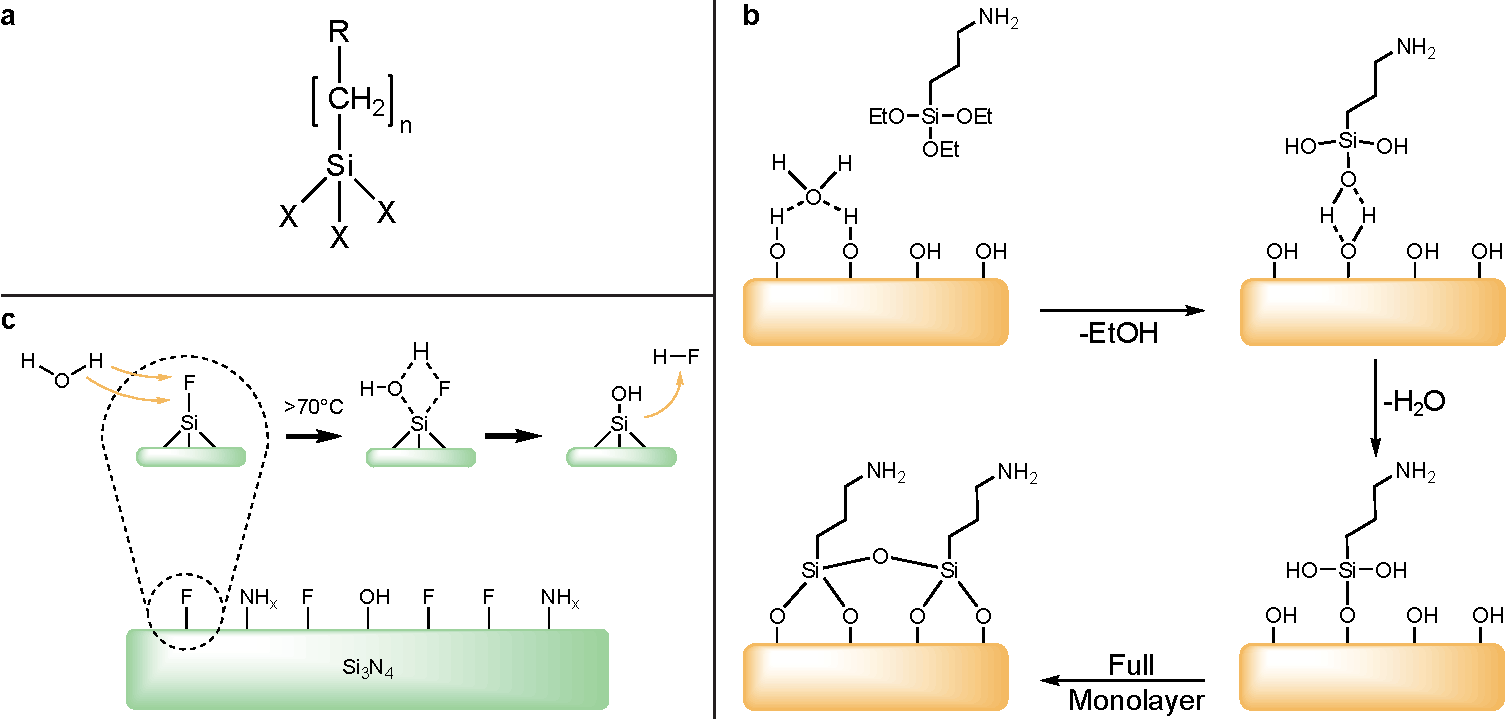
\includegraphics[width=\linewidth]{./Ressources/Chemistry/SiN-APTES-Silane.pdf}
	\capption{Surface Oxidation and Modification by APTES}{(\textbf{a}) Structure of a typical trialkoxysilane, X: hydrolyzable group, R: non-hydrolyzable organic radical, n: methylene chain-length. (\textbf{b}) Before a condensation reaction, the oxidized surface has formed hydrogen bonds with water molecules while the silane molecules are in the bulk solution. The hydrolyzed \gls{silanol} group adsorbs onto the surface and forms hydrogen bridges with the silicon bound oxygen atom. In a condensation reaction, under the loss of water, a covalent bond to the surface forms. After the \gls{sam} assembly the surface is saturated with a covalent-bound, crosslinked silane film.\cite{lit:chem:aptes:SilaneReaction} (\textbf{c}) Proposed oxidation of \gls{sin} with \gls{hf}: Due to similar activation energies water can displace \gls{hf} in a competitive manner effectively above a temperature of \SI{70}{\degreeCelsius}.}
	\label{fig:chem:APTES}
\end{figure}
The applications of organosilane modifications range from altering the adhesion characteristics and catalyzing chemical transformation at the heterogeneous interface towards ordering the interfacial region, and modifying its partition characteristics.\cite{lit:chem:Dressick,lit:chem:aptes:SilaneReview,lit:chem:surface:methods} Significantly, it includes the ability to effect a covalent bond between organic and inorganic materials. Especially in optical or biological sensors, silane modifications open a broad range of applications.\cite{lit:chem:sin:langeDiss,lit:Anti-EpCAM-PAA,lit:chem:aptes:SilaneReview}

However, the silanization reactions bear a few drawbacks which are often neglected. For instance, silane chemistry is strongly temperature and pH-dependent.\cite{lit:chem:silaizationTemp,lit:chem:silanizationParameters} Further, in a process to build \glspl{sam} from \gls{aptes}, the reaction must be catalyzed by water. But already small changes in the water content cause dramatic deviations in layer thickness.\cite{lit:chem:sin:selectivemod} Additionally, silanes can crosslink to themselves through side reactions. (\cref{fig:chem:APTES}b) \cite{lit:chem:aptes:Crosslink}



\subsection{Carbodiimide Crosslinker Chemistry}
By \gls{aptes} \gls{amine}-terminated films form the basis of many reactions and open the possibility to various applications, such as the direct attachment of biofunctional molecules by carbodiimide crosslinking chemistry.\cite{lit:bio:BioconjugateTechniques} Here, \gls{carboxyl} groups are modified by \gls{edc} and \gls{nhs} to form a stable secondary \gls{amide} bond with any primary \gls{amine}.

\begin{figure}[htb!]
	\centering
	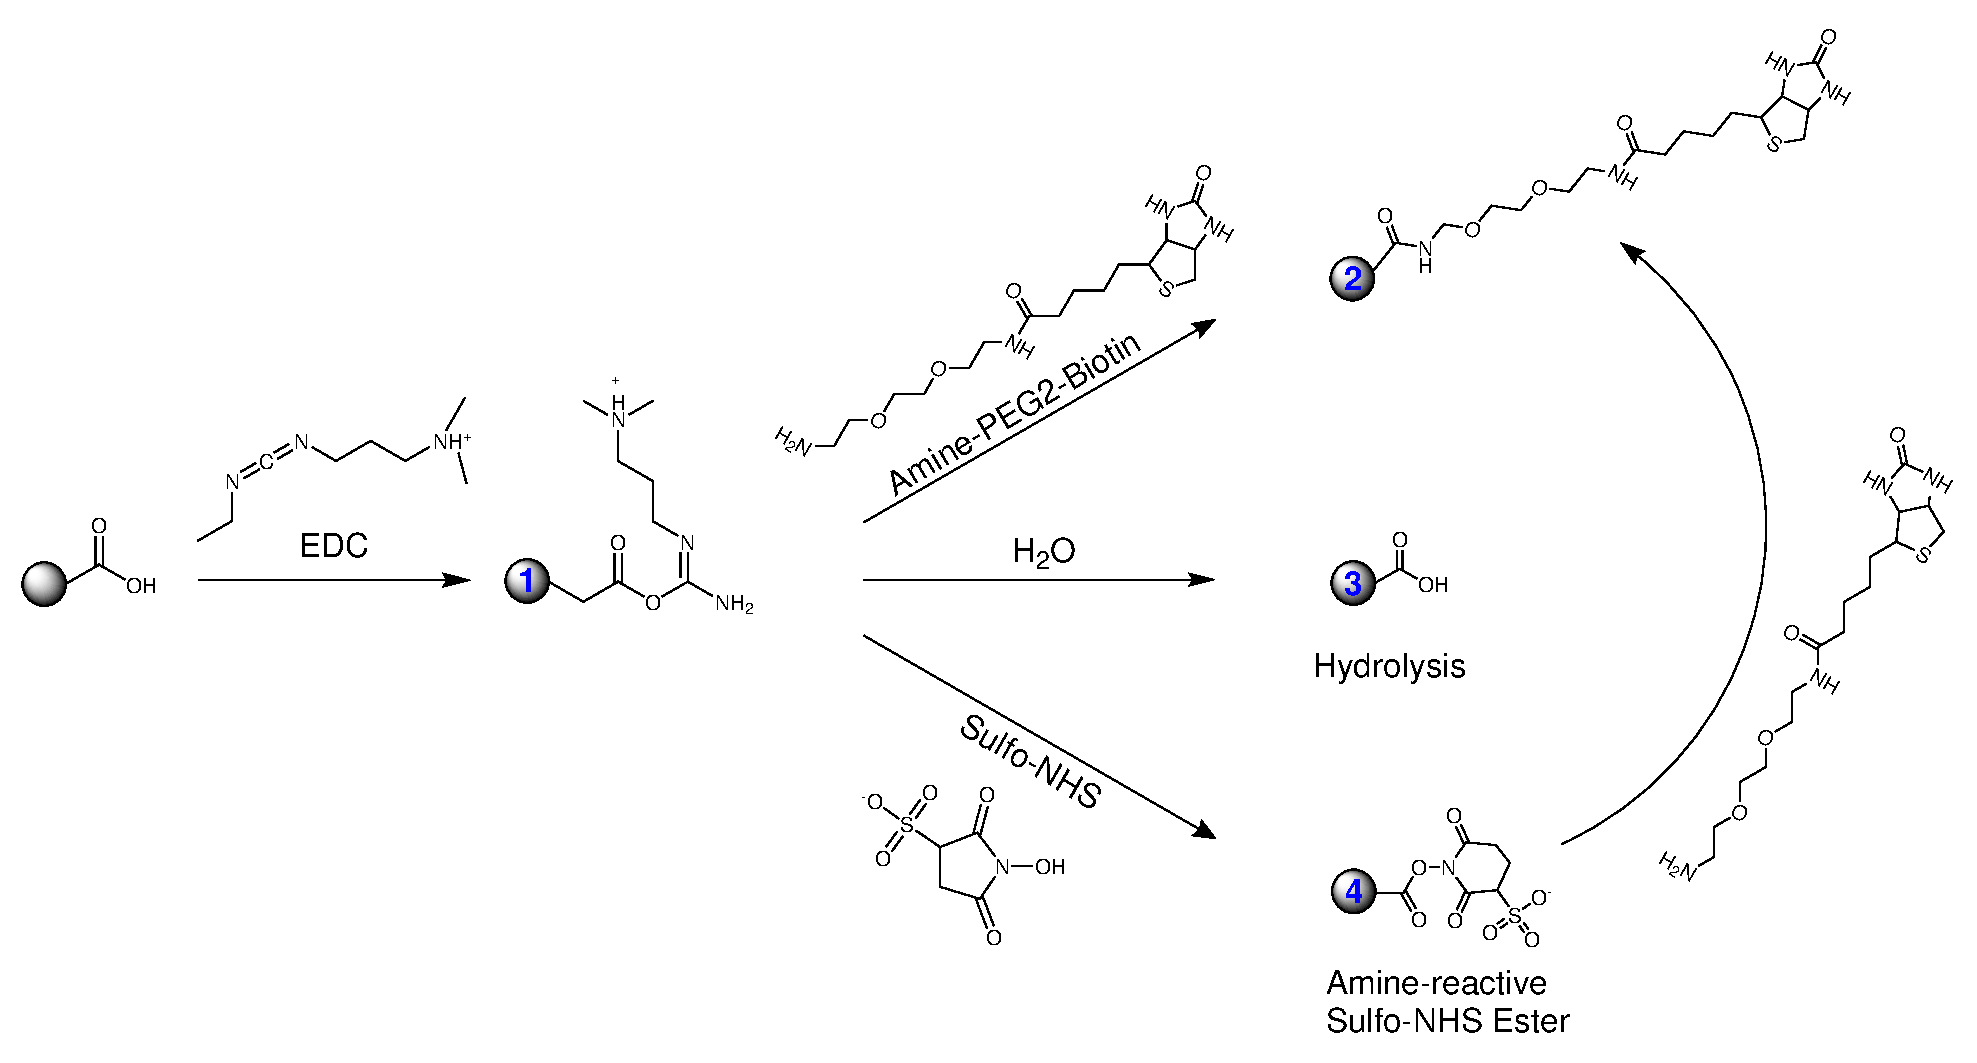
\includegraphics[width=\linewidth]{./Ressources/Chemistry/EDC-NHS.eps}
	\capption{Carboxyl bead modification with EDC/NHS}{The carboxy groups bead are activated with \gls{edc} to an active O-acylisourea intermediate. This can then either be nucleophilicly attacked by a primary amine of the amine-PEG$_2$-biotin reactant or - due to its instability - hydrolzed back to a regenerated carboxyl surface. A present NHS-ester can also displace the O-acylisourea to form a considerably more stable intermediate which then itself reacts with any primary amine.}
	\label{fig:chem:COOH-EDC-NHS}
\end{figure}
\clearpage
The general reaction mechanism is depicted in \cref{fig:chem:COOH-EDC-NHS} for the example of a particle surface, but it can equivalently be applied to any other modified surface or molecule. The initial \gls{carboxyl} group is esterified by \gls{edc} to an active o-acylisourea intermediate and leaves rapidly upon nucleophilic attack of an amine with release of an iso-urea byproduct. A zero-length amide linkage is formed. (\cref{fig:chem:COOH-EDC-NHS}, 1->2) Sulfhydryl and hydroxyl groups also will react with such active esters, but the products of such reactions, thioesters and esters, are relatively unstable compared to an \gls{amide} bond. (\cref{fig:chem:COOH-EDC-NHS}, 1)\cite{lit:bio:BioconjugateTechniques} \newline
However, this reactive complex is slow to react with amines and can hydrolyze in aqueous solutions. If the target amine does not find the active \gls{carboxyl} before it hydrolyzes (\cref{fig:chem:COOH-EDC-NHS}, 3), the desired coupling cannot occur. This is especially a problem when the target molecule is in low concentration compared to water, as in the case of protein molecules. Notwithstanding, forming a \gls{nhs} ester intermediate from the reaction of the \gls{hydroxyl} group on NHS with the \gls{edc} active-ester complex increases the resultant amide bond formation remarkably. (\cref{fig:chem:COOH-EDC-NHS}, 4->2) \cite{lit:chem:nhs2}

Another critical point in carbodiimide chemistry is the solubility of the compounds. \gls{edc}, \gls{nhs} and \gls{snhs} are soluble in aqueous and organic solvents. Nevertheless, activation  with  non-sulfonate \gls{nhs} decreases water-solubility of the modified carboxylate molecule, while activation with \gls{snhs} preserves or increases its water-solubility by virtue of the charged sulfonate group.\cite{lit:chem:snhs}

\clearpage

\subsection{The Biotin-Avidin-System}
\label{sec:theo:biotin}
Until now, the interaction of the homotetrameric protein avidin and its ligand biotin forms one of the strongest known non-covalent bonds in biological systems characterized by a \gls{kd} in the range of \SI{e-15}{\molar}.\cite{lit:bio:biotin:avidin_discovery} First isolated from chicken egg white, it became a standard to use in biotechnology when researchers found a similar bacteria protein - streptavidin - in \textit{Streptomyces} strains.\cite{lit:bio:biotin:discovery} However, the charged glycoprotein avidin exhibits unspecific binding in some assays in comparison to streptavidin. Therefor, several companies developed deglycosylated forms of avidin with a neutral isoelectric points to minimize unspecificity. (NeutrAvidin, Extravidin, NeutraLite) In recent studies, a mutant streptavidin called ``Traptavidin'' exhibitied an even 10 times dissociation rate.\cite{lit:bio:biotin:engStrep}
As discovered in the early 1990s, biotin is bound inside a highly stable $\beta$-barrel structure, and stabilized by hydrogen bonds and van der Waals forces.\cite{lit:bio:biotin:bindingmechanism} In a unique mechanism, a side group of biotin (valerate) binds to a neighboring monomer of streptavidin and therefor stabilizes the dimer complex intrinsically.\cite{lit:bio:biotin:binding,lit:bio:biotin:freeenenergy} From a thermodynamical point-of-view, the interaction of the vitamin and protein is described by a total free binding energy of \SIrange{300}{330}{\kilo\joule\per\mole} for a tetrameric protein.\cite{lit:bio:biotin:freeenenergy}  All these aspects lead to a significant rupture force for the biotin-release of \SI{200+-50}{\pico\newton}.\cite{lit:bio:biotin:rupture}

\begin{figure}[tbph!]
	\subfloat{
		\subfigimg[height=180pt]{\textbf{a}}{./Ressources/Biology/biotin.eps}
		\phantomsubcaption
		\label{fig:biotin}
	}%
	\hfill
	\subfloat{
		\centering
		\subfigimg[clip, height=180pt]{b}{Ressources/Biology/crystalAvidin_bindingSite.png}
		\phantomsubcaption
		\label{fig:crystalavidin}
	}%
	\capption{Functional Structures of Biotin and Streptavidin}{(\textbf{a}) Two- and three dimensional chemical structure of the biotin molecule. (\textbf{b}) Homotetrameric streptavidin with four subunits and four bound biotin-ligands. The molecule is attached with the anchor point at one terminus to a surface.\cite{lit:bio:SA:crystal}}
	\label{}
\end{figure}
\clearpage

\section{Magnetoresistive Sensing}
\label{sec:theo:magnet}
\begin{figure}[tbp]
	%\setlength\belowcaptionskip{-90pt}
	\centering	
	\subfloat{
		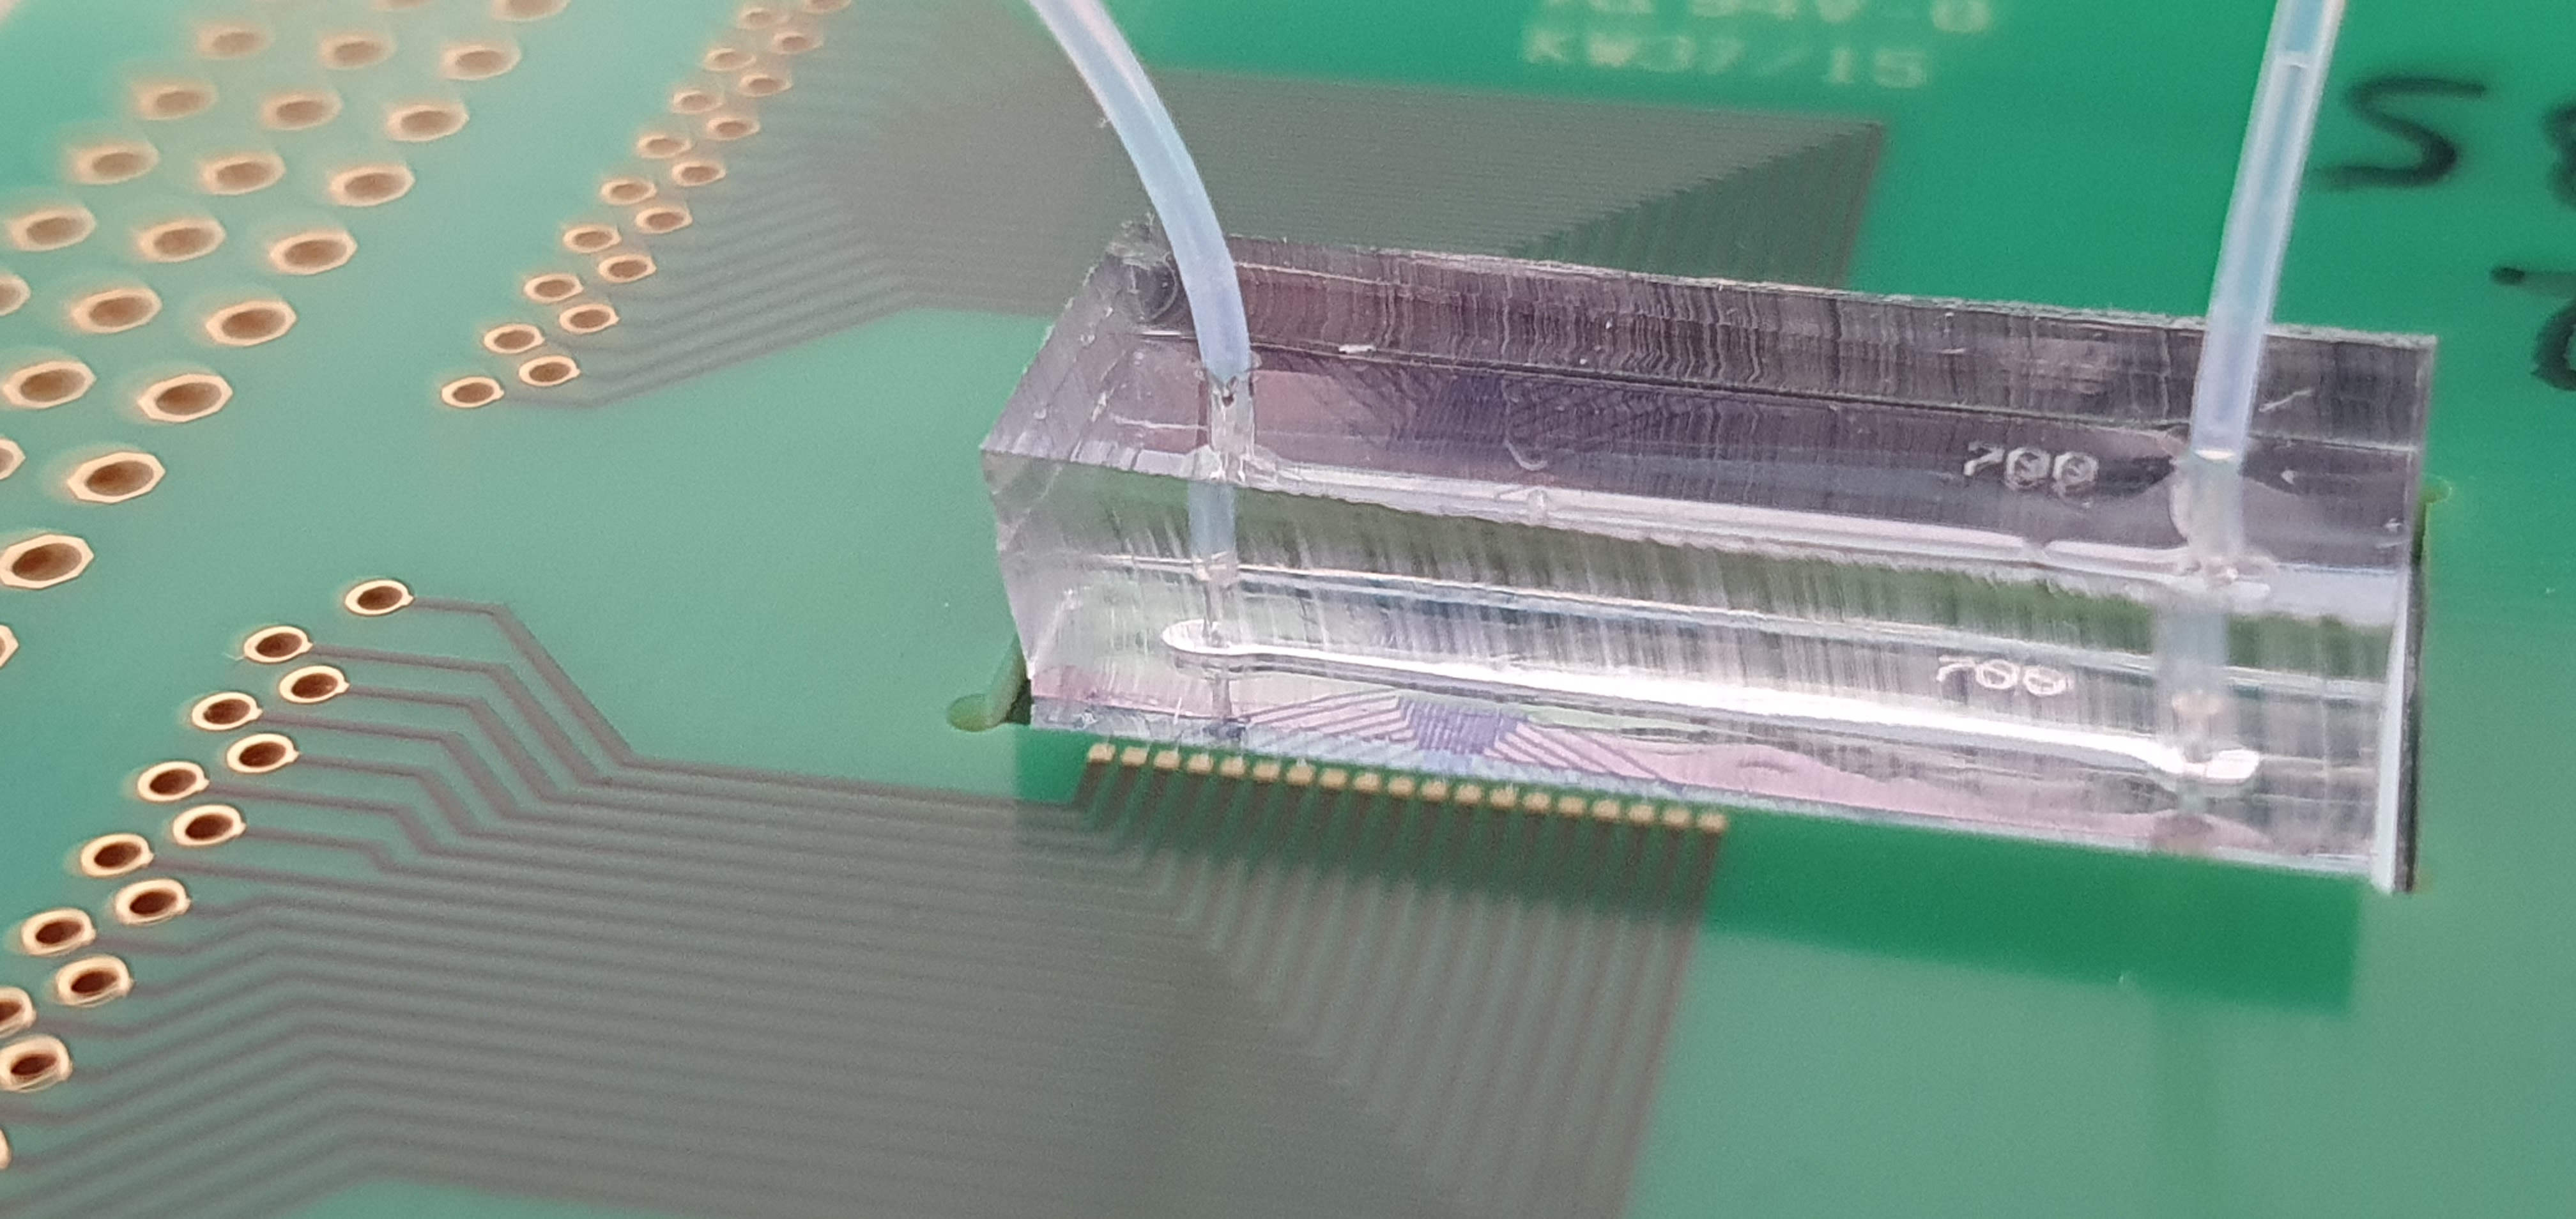
\includegraphics[width=\linewidth]{./Ressources/Electronics/chip.pdf}
	}\\
	\vspace{\baselineskip}	
	\subfloat{
		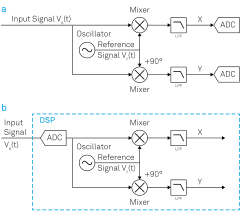
\includegraphics[height=150pt]{./Ressources/Electronics/lockin_principle}
	}%
	\hfill	
	\subfloat{
		\subfigimg[height=139.5pt]{j}{./Ressources/Electronics/mrcyte}
	}
	\capption{Overview over the MRCyte Sensor Setup}{	(\textbf{a}) Microfluidic outlet connection to waste reservoir. (\textbf{b}) Imprinted channel width. (\textbf{c}) Microfluidic inlet connection to syringe pump. (\textbf{d}) Magnetophoretic focusing region, not visible in this picture. (\textbf{e}) \Gls{gmr}-sensor region, the supply and bridge balancing traces are visible. (\textbf{f}) Gold bondpad: In order to connect the silicon sensor chip with the breakout \gls{pcb}, wedge bonds from the chip pads to the \gls{pcb} pads are forged. (\textbf{g}) Through hole plating for the connection to the lock-in via jumper cables or a soldered connector plug. (\textbf{h}) Typical signal processing flow of a lock-in. The reference signal $V_r(t)$ is splitted and mixed with the input signal with a phase difference of \ang{0} and \ang{90}. Then, both signals are low-pass filtered and sampled by an analog-to-digital converter (ADC). (\textbf{i}) Accordingly, in a digital signal processing (DSP) device the input signal is digitally converted beforehand, which in turn requires a highly sensitive and fast ADC. In contrast, DSP is more accurate and allows for software-controllable technical opportunities. (\textbf{j}) \Gls{gmr}-sensor bridge circuit inside the microfluidic channel. On the left hand side, magnetophoretic focusing structures are visible. On the right hand side, four Wheatstone bridges on a compliant ground plane can be observed.}
	\label{fig:MRCyte}	
\end{figure}

The measurement system's main component is a \gls{gmr}-sensor stack with a measured magnetoresistive effect of \textasciitilde \SI{8}{\percent}. \gls{gmr} is a quantum mechanical magnetoresistance effect observed in multilayers composed of alternating magnetic and non-magnetic conductive layers. The driving factor for this resistance is the mean free path of electrons in the interfactial regions of the soft ferromagnetic layer which is related to the spin orientation. Two ferromagnetic layers with a thin conducting, non-magnetic spacer in the center build the base of the GMR stack.\cite{lit:nano:magnetism} One ferromagnetic layer is hard magnetic\footnote{thus requires a high coercitive field to become polarized magnetically}, which is insensitive to outer magnetic fields. The so called \textit{free layer} is soft magnetic. Hence, it modulates its orientation in dependence to small coercive forces and is the main sensing component. \cite{lit:nano:Guimares2017}

In the case if both layers are aligned parallel, applying a current to the sensor allows electrons to pass through the layers with less impact into spins on either sides. Accordingly, the overall resistance is low compared to another extremum in the antiparallel alignment. The magnetization direction can be controlled, for example, by applying an external magnetic field.\cite{lit:nano:physicsmagneticmaterials, lit:nano:GMRPatent} 

In the present system, \gls{gmr} stacks were used in a Wheatstone configuration, where two resistors act as a reference for bridge balancing. Upstream to the sensor, nickel-iron-based chevron patterns act as integrated focusing based on magnetophoresis for magnetic particles. These structures are driven by an external permanent magnet hence imposing a high flux density gradient on particles. Above these patterns, previously mentioned \gls{sin} passivation has been deposited in thicknesses ranging from \SIrange{50}{500}{\nano\meter} to achieve inertness to biological samples. Nevertheless, a minimal passivation thickness is desired to measure the $r^3$-decaying magnetic field sensitive and reduce the magnetic diameter. On top of the sensor chip, a straight microfluidic channel is mounted to execute flow cytometry experiments.\cite{lit:paperHelou,lit:paperReisbeck}

In order to measure the change in resistance sensitively, the lock-in principle is used. Here, an amplifier extracts signals in a defined frequency band around a reference frequency. This efficiently filters all other frequency components. Thereby a lock-in amplifier performs a multiplication of its input $V_s(t)$ with a reference signal $V_r(t)$ and low-pass filters the result $Z(t)$. In most integrated cases, the reference signal is generated additionally by the lock-in amplifier itself. Using a pure sine wave as reference enables a selective measurement at the fundamental frequency or its harmonics.\cite{lit:nano:lockin} 

At a measurement, $V_s(t)$ is split and separately multiplied with the reference signal and a \ang{90} phase-shifted copy of it. After demodulation, the result is constituted from signal components at the sum and the difference of signal and the reference frequency, $\omega_{s}$ and $\omega_{r}$, respectively.(\cref{eq:el:sig,eq:el:ref,eq:el:result}) In the resulting signal, the trigonometric functions are Euler transformed and the magnitude $R=\sqrt{X(t)^2+Y(t)^2}$ acts as measurand. The high frequency compounds are then filtered digitally by a low-pass filter of varying order $n$ to increase \gls{snr}. As described in \cref{eq:el:filter}, a low-pass in the frequency domain can be described by a power series of first-order filters.

\begin{align}
		V_{s}(t) &=\sqrt{2} R \cdot \cos \left(\omega_{s} t+\Theta\right) \label{eq:el:sig} \\
	V_{r}(t)&=\sqrt{2} e^{-i \omega_{r} t}=\sqrt{2} \cos \left(\omega_{r} t\right)-i \sqrt{2} \sin \left(\omega_{r} t\right) \label{eq:el:ref}\\
	Z(t) &=X(t)+i Y(t)=V_{s}(t) \cdot V_{r}(t) \label{eq:el:result} \\
		&=R\left[e^{i\left(\left(\omega_{z}-\omega_{r}\right) t+\theta\right]}+e^{-i\left[\left(\omega_{z}+\omega_{r}\right) t+\theta\right]}\right] \\
		H_{n}(\omega)&=H_{1}(\omega)^{n}=\left(\frac{1}{1+i \omega \tau}\right)^{n} \label{eq:el:filter}
\end{align}


However, with this measurement principle \gls{snr} can not increase infinitely. If the signal strength cannot be increased, the noise  has to be reduced or avoided as much as possible. Nevertheless, noise is always caused by different sources in analog signals, for example thermal, shot, and flicker noise. Other sources are of technical origin, as for example ground loops, crosstalk, \SI{50}{\hertz} noise or electromagnetic pick-up. Predominantly, field aberrations or misalignment of the permanent magnet cause magnetic noise which dominates here.\cite{lit:nano:lockin}

Now, to characterize a \gls{gmr} with the lock-in, the free magnetization layer has to be confined in parallel and antiparallel configuration to the reference layer. For this, Helmholtz coils impose a magnetic field in \ang{+-90} of the free magnetization in order to measure the respective resistance. The lock-in captures a hysteresis during the sweep from parallel to anti-parallel alignment of the layers at a specific bridge circuit. The steepness hereby indicates the sensitivity of the sensor element in the units \si{\volt\per\tesla}.



